\documentclass[onlytextwidth]{beamer}
\usepackage[utf8]{inputenc}
\usepackage{microtype}
\usepackage{amsmath}
\usepackage{amssymb}
\usepackage[nomessages]{fp} %\FPeval{\var-name}{2*sin(pi/6)}
\usepackage{siunitx} %units in math. eg 20\milli\meter
\usepackage{yhmath} % for arcs, overparenth command
\usepackage{tikz} %graphics
\usetikzlibrary{quotes, angles}
%\usepackage{graphicx} already loaded by beamer class
%consider setting \graphicspath{{images/}}
%\parskip ?? to avoid paragraph indent
\usepackage{multicol} %may not need this package, just columns environment
\usepackage{venndiagram}

\subtitle[BECA]{Bronx Early College Academy}
\author[Huson]{Christopher J. Huson PhD}

\setbeamertemplate{headline}{\vskip2mm 
  BECA / \insertshortauthor \, / \inserttitle
  \hfill 
  \insertsection
  }

\title{Geometry Unit 1, part b: Area}
\date{19-23 September 2022}

\begin{document}
\frame{\titlepage}

\section[Outline]{}
\frame{\tableofcontents}

\section{1.8 Area \hfill 19 September}
\begin{frame}{Learning Target: I can calculate areas}
  {CCSS: HSG.CO.A.1 Know precise geometric definitions \hfill \alert{1.8 Monday 19 Sept}}
  \begin{block}{Do Now: Practice unit conversion}
    \begin{enumerate}
        \item How many days are in a week?
        \item Find the number of weeks in 365 days. \par (show calculation with units)
    \end{enumerate}
    \end{block} \vspace{3cm}
    Quiz results \par \medskip
    Lesson: Rectangle, triangle, parallelogram area formulas \par \medskip
    Extension: Scientific notation
  \end{frame}

\begin{frame}{The \emph{area} of a rectangle is its base $\times$ height.}
    {We also say ``length times width''}
    Formula for the area of a rectangle:
    {\large $$A=b \times h$$}
        \begin{columns}
            \column{0.5\textwidth}
            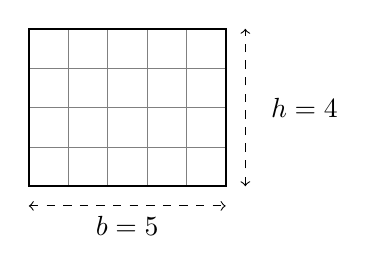
\begin{tikzpicture}[scale=.5]
                \draw[help lines] (0,0) grid (5,4);
                \draw[thick] (0,0)--(5,0)--(5,4)--(0,4)--cycle;
                \draw[<->, dashed] (0,-0.5)--(5,-0.5);
                \node at (2.5, -1){$b=5$};
                \draw[<->, dashed] (5.5,0)--(5.5,4);
                \node at (7, 2){$h=4$};
            \end{tikzpicture}
            \column{0.5\textwidth}
            $$A = 5 \times 4 = 20$$
        \end{columns} \vspace{1.5cm}
        \begin{description}
            \item[Area] the quantity of unit squares that fill a shape
        \end{description}
    \end{frame}

\begin{frame}{A parallelogram's area has the same formula as a rectangle.}
    {Use the height, not the length of the slanted side.}
    Formula for the area of a parallelogram:
    {\large $$A=b \times h$$}
        \begin{columns}
            \column{0.5\textwidth}
            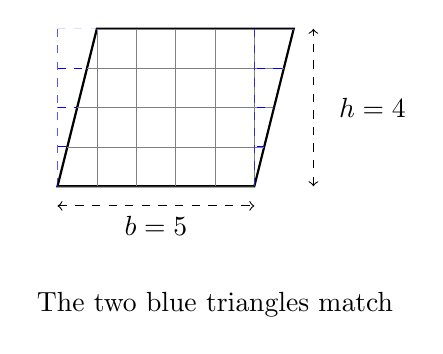
\begin{tikzpicture}[scale=.5]
                \draw[thick] (0,0)--(5,0)--(6,4)--(1,4)--cycle;
                \draw[<->, dashed] (0,-0.5)--(5,-0.5);
                \node at (2.5, -1){$b=5$};
                \draw[<->, dashed] (6.5,0)--(6.5,4);
                \node at (8, 2){$h=4$};
                \begin{scope}
                    \clip (0,0)--(5,0)--(6,4)--(1,4)--cycle;
                        \draw[help lines] (0,0) grid (6,4);
                \end{scope}
                \onslide<2>
                    \begin{scope}
                        \clip (0,0)--(1,4)--(0,4)--cycle;
                        \draw[dashed, blue] (0,0) grid (6,4);
                    \end{scope}
                    \begin{scope}
                        \clip (5,0)--(6,4)--(5,4)--cycle;
                        \draw[dashed, blue] (0,0) grid (6,4);
                    \end{scope}
                    \node at (4,-3){The two blue triangles match};
            \end{tikzpicture}
            \column{0.5\textwidth}
            $$A = 5 \times 4 = 20$$
        \end{columns} \vspace{1.5cm}
    \end{frame}

\begin{frame}{A triangle has half the area of its base times height.}
    {Use the triangle's height or \emph{altitude}, not the side length.}
    Formula for the area of a triangle:
    {\large $$A= \frac{1}{2} b \times h$$}
        \begin{columns}
            \column{0.5\textwidth}
            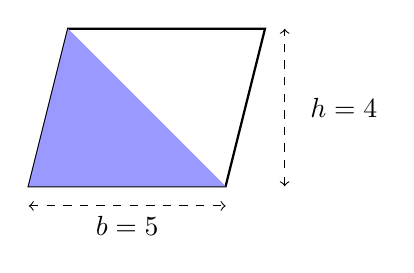
\begin{tikzpicture}[scale=.5]
                \draw[thick] (0,0)--(5,0)--(6,4)--(1,4)--cycle;
                \draw[<->, dashed] (0,-0.5)--(5,-0.5);
                \node at (2.5, -1){$b=5$};
                \draw[<->, dashed] (6.5,0)--(6.5,4);
                \node at (8, 2){$h=4$};
                \fill[blue!40] (0,0)--(5,0)--(1,4)--cycle;
            \end{tikzpicture}
            \column{0.5\textwidth}
            $$A =  \frac{1}{2} (5 \times 4) = 10$$
        \end{columns} \vspace{1.5cm}
        \begin{description}
            \item[Altitude] The height of a triangle (distance $\perp$ to its base)
        \end{description}
    \end{frame}

\begin{frame}{Find a missing dimension using the area formula}
    Given the area of a triangle is 40 and its base is 10, find its height. \vspace{1cm}
    \begin{columns}
        \column{0.5\textwidth}
        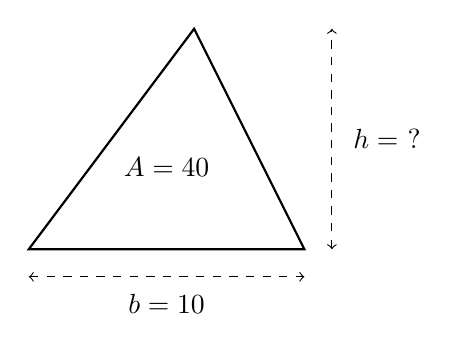
\begin{tikzpicture}[scale=.7]
            \draw[thick] (0,0)--(5,0)--(3,4)--cycle;
            \draw[<->, dashed] (0,-0.5)--(5,-0.5);
            \node at (2.5,-1){$b=10$};
            \draw[<->, dashed] (5.5,0)--(5.5,4);
            \node at (6.5,2){$h=$ ?};
            \node at (2.5,1.5){$A=40$};
        \end{tikzpicture}
        \column{0.5\textwidth}
        $$A =  \frac{1}{2} (10 \times h) = 40$$
    \end{columns} \vspace{1.5cm}
    \end{frame}

\begin{frame}{Write formulas in notebook}
        \begin{description}
            \item[Rectangle] $A=b \times h$ (base times height or length times width)
            \item[Parallelogram] $A=b \times h$
            \item[Triangle] $A=\frac{1}{2} (b \times h)$ \vspace{0.5cm}
            \item[Area] the quantity of unit squares that fill a shape
            \item[Units] We say ``square units'', i.e. square inches (abbreviated $\text{in}^2$), square miles, etc.
            \item[Altitude] Height (distance $\perp$ to the baseline)
        \end{description}
    \end{frame}
    
\begin{frame}{Extension (optional): \emph{Scientific notation}}
    {Use for very large or small numbers instead of decimals}
    Exponents mean repeated multiplication:
        $$10^5 = 10 \times 10 \times 10 \times 10 \times 10 = 100,000$$
    \begin{enumerate}
        \item The distance to the sun is 150,000,000,000 meters $=1.5 \times 10^{11}$
        \item The population of NYC is $8,000,000 = $ \bigskip
        \item The area of the earth is $2 \times 10^{8}$ square miles $=$
    \end{enumerate} \bigskip
    \begin{description}
        \item[Scientific notation] Compact notation for big numbers, $a \times 10^k$
        \item[Exponent] Repeated multiplication. The number of decimal places in base 10
        \item[Base 10] The system of place value we use for numbers
        \item[Mantissa] The coefficient in scientific notation
    \end{description}
    \end{frame}

\section{1.9 Rounding and circle area \hfill 20 September}
\begin{frame}{Learning Target: I can calculate the area of a circle}
    {CCSS: HSG.CO.A.1 Know precise geometric definitions \hfill \alert{1.9 Tuesday 20 Sept}}
        Do Now: Two rectangles are shown. Calculate the area of each and the combined total area.
        \begin{flushleft}
            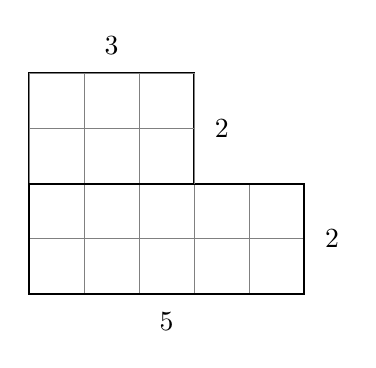
\begin{tikzpicture}[scale=.7]
                \draw[help lines] (0,0) grid (5,2);
                \draw[thick] (0,0)--(5,0)--(5,2)--(3,2)--(3,4)--(0,4)--cycle;
                \draw[help lines] (0,2) grid (3,4);
                \draw[thick] (0,2)--(3,2);
                \node at (5.5,1){2};
                \node at (3.5,3){2};
                \node at (2.5,-0.5){5};
                \node at (1.5,4.5){3};
            \end{tikzpicture}
          \end{flushleft}
        Lesson: Area of a circle, $\pi$, rounding \par \medskip
        Extension: Significant figures
    \end{frame}

\begin{frame}{The \emph{area} and  \emph{circumference} of a circle are multiples of $\pi$.}
    {$\pi$ is an \emph{irrational number}}
    \begin{columns}
        \column{0.5\textwidth}
            Area of a circle:
            {\large $$A=\pi r^2$$}
        \column{0.5\textwidth}
            Circumference (distance around):
            {\large $$C=2 \pi r$$}
        \end{columns}  \vspace{0.5cm}
        \begin{columns}
            \column{0.5\textwidth}
            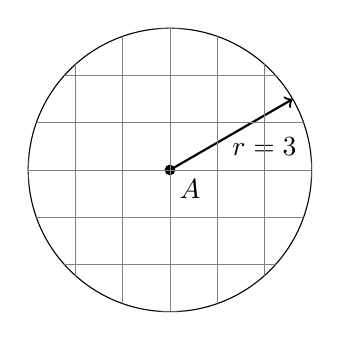
\begin{tikzpicture}[scale=.6]
                \draw (0,0) circle [radius=3];
                \draw[fill] (0,0) circle [radius=0.1] node[below right]{$A$};
                \draw[thick, -{>[scale=1.5]}] (0,0)--(30:3);
                \node at (2,0.5){$r=3$};
                \clip (0,0) circle [radius=3];
                  \draw[help lines] (-4,-4) grid (4,4);
              \end{tikzpicture}
            \column{0.5\textwidth}
            Circle $A$ with radius $r=3$
            $$A = \pi \times 3^2 = 9 \pi = 28.2743... $$
            $$C = 2\pi \times 3 = 6 \pi = 18.8495... $$
        \end{columns} \vspace{0.5cm}
        \begin{description}
            \item[Radius] Segment from the center to the edge of a circle, $r$
            \item[Diameter] Segment/length across the whole circle, $D=2r$
        \end{description}
    \end{frame}

\begin{frame}{Numbers don't always need to be exact}
    Round up when the next digit is 5 or more \par 
    Round down otherwise \par
    \onslide<1> {\hspace{4cm}Is $\pi$ closer to three or four?} \par
        $\pi = 3.{\color{red}1}415926... $
    \onslide<2-> $\approx 3$ to the nearest whole number
    \onslide<3-> $\pi = 3.1{\color{red}4}15926... \approx 3.1$ to the nearest tenth \par
        $\pi = 3.14{\color{red}1}5926... \approx 3.14$ to the nearest hundredth \par
        $\pi = 3.141{\color{red}5}926... \approx 3.14{\textbf 2}$ to the nearest thousandth \bigskip
    \onslide<4-> 
        \begin{description}
        \item[Whole] The ones place, e.g. 3, 14, -15
        \item[tenths] First digit after the decimal, 0.3, 6.8
        \item[hundredths] Second decimal digit, 5.45
        \item[thousandths] Third decimal place, 18.123
        \item[Rounding] Writing an approximation of a number
        \item[Approximate] About equal to, not exact, $\approx$
    \end{description}
    \end{frame}

\begin{frame}{Use the symbol $\pi$ for an \emph{exact} answer}
    \begin{columns}
        \column{0.4\textwidth}
        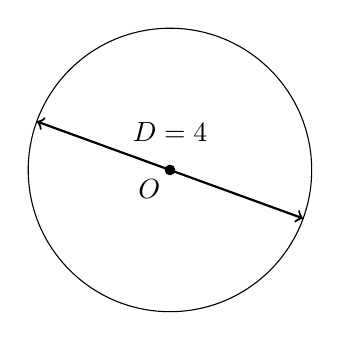
\begin{tikzpicture}[scale=.6]
            \draw (0,0) circle [radius=3];
            \draw[fill] (0,0) circle [radius=0.1] node[below left]{$O$};
            \draw[thick, <->] (160:3)--(-20:3); %{<->[scale=1.5]}
            \node at (0,0.8){$D=4$};
            \end{tikzpicture}
        \column{0.6\textwidth}
        Circle $O$ with diameter $D=4$
        \begin{enumerate}
            \item Find the radius of the circle. \par \medskip
            \onslide<2->  {$r = \frac{1}{2}D = \frac{4}{2} =2 $} \medskip
            \item Find the exact circumference. \par \medskip
            \onslide<3->  {$C = 2 \pi r = 2 \pi 2 = 4 \pi $} \medskip
            \item Round to the nearest hundredth. \par \medskip
            \onslide<4>  $C = 4 \pi = 12.56{\color{red}6}3706... \approx 12.57 $
        \end{enumerate}
    \end{columns} \vspace{2cm}
    \begin{description}
        \item[Exact solution] Written with symbols or an ellipse ($...$). \par 
        Also said as ``give your answer \emph{in terms of} $\pi$''.
    \end{description}
    \end{frame}
    
\begin{frame}{Write formulas in notebook}
    \begin{description}
        \item[Circle] All points with equal distance from the circle center
        \item[Radius] Distance from the circle center to its edge, $r$
        \item[Diameter] Length across the whole circle, $D=2r$        
        \item[Circle area] Formula $A=\pi r^2$
        \item[Circumference] The distance around a circle (i.e. perimeter), $C=2\pi r$
        \item[Semi-circle] Half of a circle
        \item[{\Large $\pi$}] A special number, $\pi = 3.14159265358...$
        \item[Irrational] Number that can not be written as a fraction, $\pi$, $\sqrt{2}$
        \item[Exact solution] Written with symbols or an ellipse ($...$). \par 
        Also said as ``give your answer \emph{in terms of} $\pi$''.
        \end{description}
    \end{frame}

\begin{frame}{Extension: Three digits is usually exact enough}
    {Scientists and engineers say \emph{significant figures}, or in IB, ``sig figs''}
    Round to three digits
    \begin{itemize}
        \item $\pi = 3.14159265358... \approx 3.14$
        \item $\sqrt{2}= 1.4142135... \approx 1.41$
        \item Dr. Huson's height $h \approx 67.5$ inches
        \item 365 days in a year (actually 365.2421897, \href{https://www.math.net/days-in-a-year}{source})
        \item Avogadro's number $N_A \approx 6.02 \times 10^{23}$
    \end{itemize} \vspace{1cm}
    \begin{description}
        \item[Sig figs] Significant figures, the number of digits required for the desired precision. In IB mathematics and most practical matters, the convention is 3 sig figs.
    \end{description}
    \end{frame}


\section{1.10 Precision \hfill 21 September}
\begin{frame}{Learning Target: I can quantify error in calculations}
    {CCSS: HSG.CO.A.1 Know precise geometric definitions \hfill \alert{1.10 Wednesday 21 Sept}}
        Do Now: Find the area of a quarter circle with radius $r=20$ cm, rounding to the nearest whole number. \par \bigskip
        \begin{columns}
            \column{0.3\textwidth}
            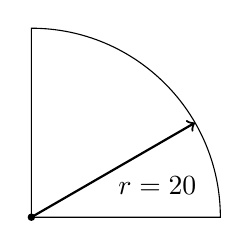
\begin{tikzpicture}[scale=.8]
                \draw (0,0)--(3,0) arc (0:90:3)--cycle;
                \draw[fill] (0,0) circle [radius=0.05];
                \draw[thick, -{>[scale=1.5]}] (0,0)--(30:3);
                \node at (2,0.5){$r=20$};
              \end{tikzpicture}
            \column{0.7\textwidth}
            \onslide<2->
            $A = \frac{1}{4} \pi \times 20^2 = 100 \pi$ \par \bigskip
            $= 314.15926... \approx 314 \text{ square units}$
        \end{columns} \vspace{1cm}
        \onslide<1->
        Lesson: Percent error formula \par \medskip
        Extension: Confidence intervals
    \end{frame}  

\begin{frame}{Quantify measurement and rounding inaccuracy as a percent}
    {Convention: Treat all errors as a positive amount}
    Given $v_A= \text{Approximate value}$, $v_E= \text{Exact value}$ \par \bigskip
    Percent error
    $$\epsilon = \left|\frac{v_A-v_E}{v_E}\right| \times 100\%$$
    \bigskip    
    Which is more accurate? %\bigskip
        \begin{columns}
            \column{0.4\textwidth}
                $\pi \approx 3.14$ \par \bigskip
                \onslide<2>{$\epsilon=\left|\frac{3.14-\pi}{\pi}\right| \times 100\%$ \par \medskip $ = 0.05069...\%$}
            \column{0.6\textwidth}
                $\pi \approx \frac{22}{7}$ (\href{https://en.wikipedia.org/wiki/Archimedes}{Archimedes c. 250 B.C.}) \par \medskip
                \onslide<2>{$\epsilon=\left|\frac{22/7-\pi}{\pi}\right| \times 100\%$ \par \medskip $ = 0.04024...\%$}
        \end{columns}  \vspace{0.5cm}
        \begin{description}
            \item[Relative error] decimal format (i.e. $5\%$ versus 0.05)
            \item[$\epsilon$] The Greek letter epsilon, meaning error
        \end{description}
    \end{frame}
    
\begin{frame}{Unit conversions are often approximate}
    {39.3701 inches is a more exact value}
    There are approximately 39 inches in a meter.
    $$ 1 \text{ meter} \approx 39 \text{ inches}$$
    Find the percent error in this conversion ratio. \vspace{1cm}
    \onslide<2>
    $$\epsilon = \left|\frac{39-39.3701}{39.3701}\right| \times 100\%$$
    $$=0.940053492...\% \approx 1\% \text{ error}$$
    \end{frame}

\begin{frame}{Quantify an error as interval around the best guess}
   \begin{itemize}
    \item What is a typical retirement age? $65 \pm 5 \text{ years}$
    \item SUNY New Paltz SAT scores are between 1070 and 1260.
    \item How much does it rain in New York City? 
        \href{https://weatherspark.com/y/23912/Average-Weather-in-New-York-City-New-York-United-States-Year-Round\#Figures-Rainfall}{(WeatherSpark)}
   \end{itemize}
     \center{\textit{Average Monthly Rainfall in New York City} \par
        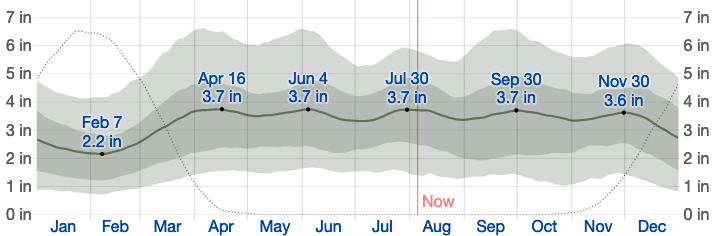
\includegraphics[height=4cm]{../graphics/rainfall.png}}
        \begin{description}
            \item[Interval] A range, e.g. from 10 to 12
            \item[Confidence] Not certain, but most likely range of values
            \item[$\pm$] Plus or minus
        \end{description}
    \end{frame}
    
\section{1.11 Review \hfill 22 September}
\begin{frame}{Learning Target: I can study together with my classmates}
    {CCSS: HSG.CO.A.1 Know precise geometric definitions \hfill \alert{1.11 Thursday 22 Sept}}
        Do Now: Estimate the percentage of the square's area covered by the circe. (then calculate your percent error) \bigskip
        \begin{columns}
            \column{0.4\textwidth}
            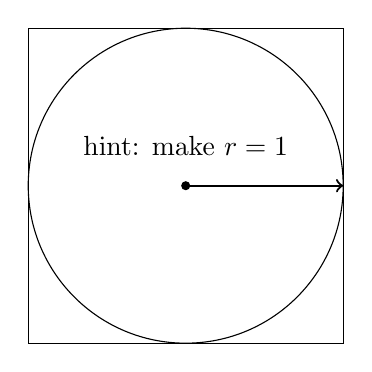
\begin{tikzpicture}[scale=1]
                \draw (-2,-2) rectangle (2,2);
                \draw (0,0) circle [radius=2];
            \onslide<2>
                \draw[fill] (0,0) circle [radius=0.05];
                \draw[thick, -{>[scale=1.5]}] (0,0)--(0:2);
                \node at (0,0.5){hint: make $r=1$};
              \end{tikzpicture}
    \column{0.6\textwidth}
    \onslide<2>{ Guestimating three quarters, or $75\%$ \par \bigskip
        \hspace{0.4cm} $A_{square} = 2 \times 2 = 4$ \par \medskip
        \hspace{0.5cm} $A_{circle} = \pi \times 1^2 = \pi = 3.14159... $ \par \medskip
        $\text{\% coverage}= \frac{\pi}{4} = 0.78539... \approx 78.5\%$ \par \medskip
        $\epsilon = \left| \frac{75 - 78.539...}{78.539...} \right| \times 100\%$  \par \medskip 
        \hspace{0.5cm} $= 4.5070...\% \approx 4.5\% \text{ error}$}
        \end{columns} \bigskip
        Lesson: Peer review, notebook check, homework inventory due \par \smallskip
        \alert{Unit test tomorrow}
    \end{frame} 

\begin{frame}{Groupwork review for \alert{test tomorrow}}
    {``Roundtable'' of four students, with four topics assigned}
    \begin{block}{Geometry skills to study / teach}
        \begin{enumerate}
        \item Line segments, length, number lines
        \item Perimeter and area
        \item Precision, percent error
        \item Modeling situations and solving with algebra
    \end{enumerate}
    \end{block}
    \end{frame}
    
\section{1.12 Unit test: Segments, length, area \hfill 23 September}
\begin{frame}{Learning Target: I can quantify length and area}
    {CCSS: HSG.CO.A.1 Know precise geometric definitions \hfill \alert{1.12 Friday 23 Sept}}

        \alert{Unit test}
    \end{frame} 
    
    
\end{document}